\documentclass[border=12pt]{standalone}
\usepackage{amsmath}
\usepackage{tikz}
\usetikzlibrary{shapes.geometric, arrows.meta, positioning}
\begin{document}
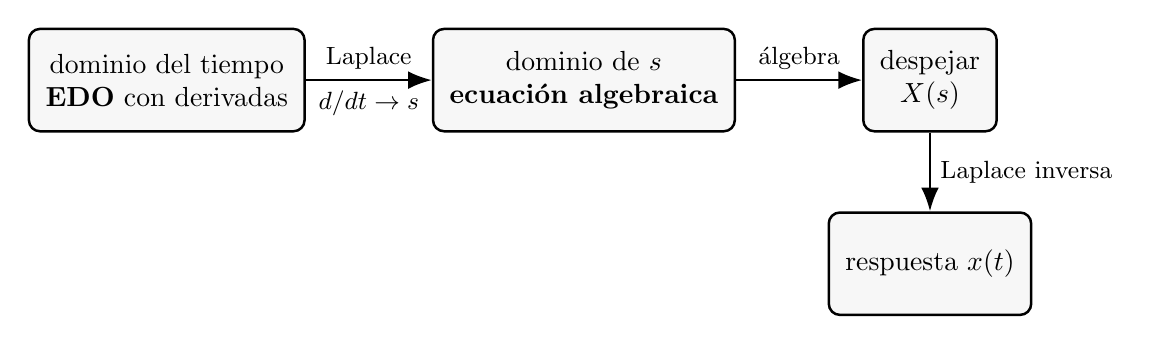
\begin{tikzpicture}[line width=0.9pt, node distance=6mm,
   box/.style={draw, rounded corners, align=center, minimum height=1.3cm, inner sep=6pt, fill=black!3},
   ar/.style={-{Latex[length=3mm]}, thick}]
  \node[box] (t1) {dominio del tiempo\\ \textbf{EDO} con derivadas};
  \node[box, right=16mm of t1] (s1) {dominio de $s$\\ \textbf{ecuación algebraica}};
  \node[box, right=16mm of s1] (s2) {despejar\\ $X(s)$};
  \node[box, below=10mm of s2] (t2) {respuesta $x(t)$};
  \draw[ar] (t1) -- node[above]{\small Laplace} node[below]{\small $d/dt\to s$} (s1);
  \draw[ar] (s1) -- node[above]{\small álgebra} (s2);
  \draw[ar] (s2) -- node[right]{\small Laplace inversa} (t2);
\end{tikzpicture}
\end{document}
